\chapter{The Execute Pipeline}\label{chapter:execute}

%when wakeup occurs?

The Execution Pipeline covers the execution and write-back of micro-ops.  Although the micro-ops will travel down the pipeline one after the other (in the order they have been issued), the micro-ops themselves are likely to have been issued to the Execution Pipeline out-of-order. Figure \ref{fig:execute-pipeline} shows an example Execution Pipeline for a dual-issue BOOM. 

\begin{figure}[htbp]
	\centering
	\centerline{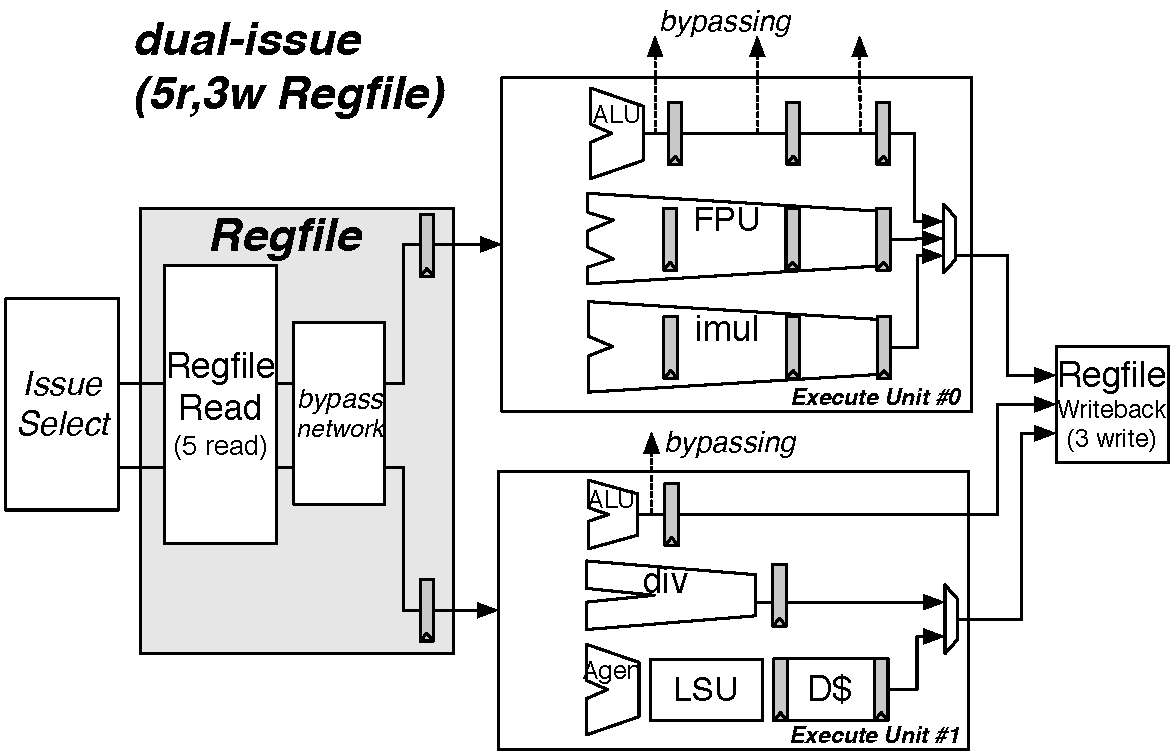
\includegraphics[scale =0.75] {figures/execution-pipeline-2w}}
	\caption{ \small An example pipeline for a dual-issue BOOM. The first issue port schedules micro-ops onto Execute Unit \#0, which can accept ALU operations, FPU operations, and integer multiply instructions.  The second issue port schedules ALU operations, integer divide instructions (unpipelined), and load/store operations.  The ALU operations can bypass to dependent instructions.  Note that the ALU in EU\#0 is padded with pipeline registers to match latencies with the FPU and iMul units to make scheduling for the write-port trivial. Each Execution Unit has a single issue-port dedicated to it but contains within it a number of lower-level Functional Units.}
	\label{fig:execute-pipeline}
\end{figure}



\section{Execution Units}


\begin{figure}[htbp]
	\centering
	\centerline{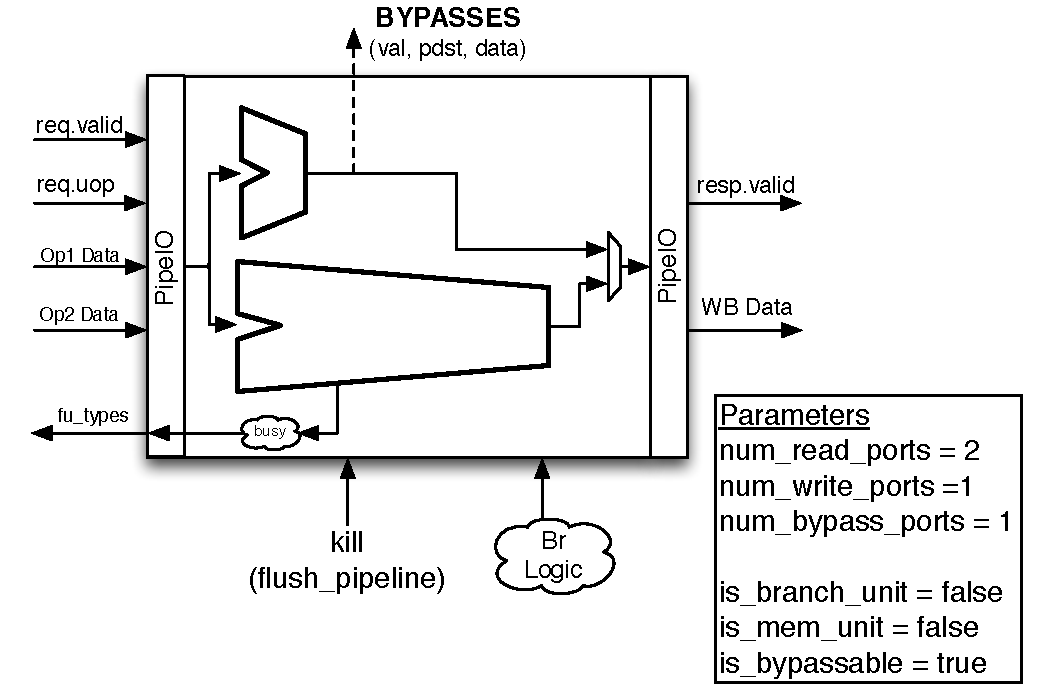
\includegraphics[scale =0.8] {figures/execution-unit}}
	\caption{ \small An example Execution Unit. This particular example shows an integer ALU (that can bypass results to dependent instructions) and an unpipelined divider that becomes {\em busy} during operation. Both functional units share a single write-port.  The Execution Unit accepts both {\em kill} signals and {\em branch resolution} signals and passes them to the internal functional units as required.}
	\label{fig:execute-unit}
\end{figure}


An Execution Unit is a module that a single issue port will schedule micro-ops onto and contains some mix of functional units.  Phrased in another way, each issue port from the Issue Window talks to one and only one Execution Unit. An Execution Unit may contain just a single simple integer ALU, or it could contain a full complement of floating point units, a integer ALU, and an integer multiply unit.  

The purpose of the Execution Unit is to provide a flexible abstraction which gives a lot of control over what kind of Execution Units the architect can add to their pipeline

\subsection{Scheduling Readiness}

An Execution Unit provides a bit-vector of the functional units it has available to the issue scheduler. The issue scheduler will only schedule micro-ops that the Execution Unit supports.  For functional units that may not always be ready (e.g., an un-pipelined divider), the appropriate bit in the bit-vector will be disabled (See Fig \ref{fig:execute-unit}).



\section{Functional Units}

Functional units are the muscle of the CPU, computing the necessary operations as required by the instructions.  Functional units typically require a knowledgable domain expert to implement them correctly and efficiently.  


\begin{figure}[htbp]
	\centering
	\centerline{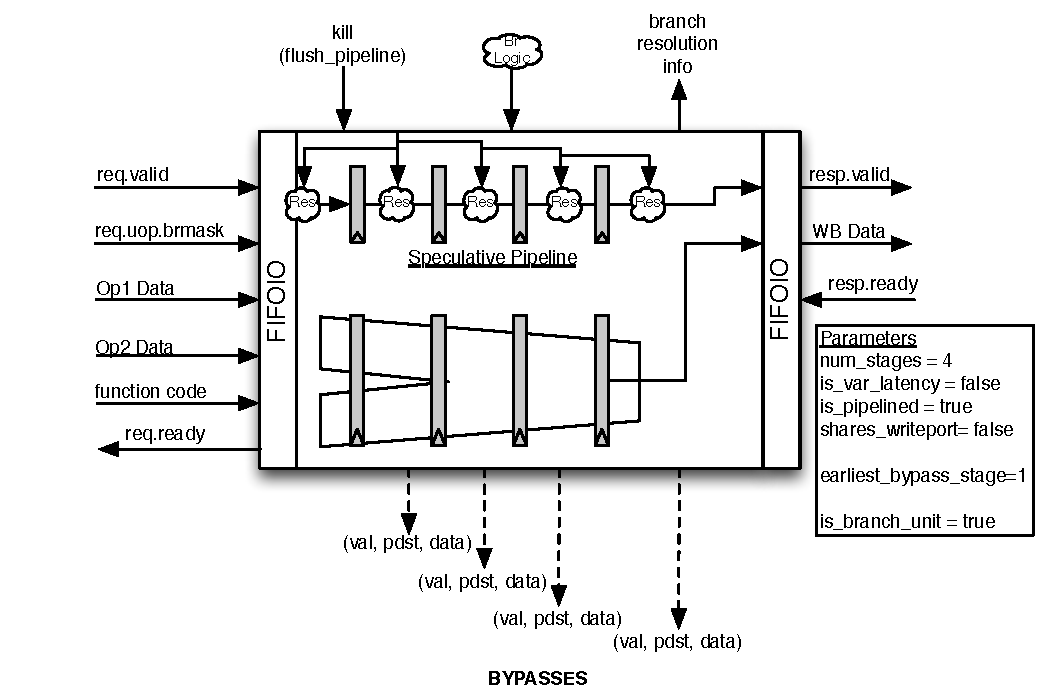
\includegraphics[scale =0.9] {figures/abstract-functional-unit}}
	\caption{ \small The abstract Pipelined Functional Unit class. An expert-written, low-level functional unit is instantiated within the Functional Unit. The request and response ports are abstracted and bypass and branch speculation support is provided. Micro-ops are individually killed by gating off their response as they exit the low-level functional unit.}
	\label{fig:abstract-functional-unit}
\end{figure}


For this reason, BOOM uses an abstract Functional Unit class to ``wrap" expert-written, low-level functional units from the Rocket repository (see Section \ref{sec:rocket}).  However, the expert-written functional units created for the Rocket in-order processor make assumptions about in-order issue and commit points (namely, that once an instruction has been dispatched to them it will never need to be killed). These assumptions break down for BOOM.

However, instead of re-writing or forking the functional units, BOOM provides an abstract Functional Unit class (see Fig \ref{fig:abstract-functional-unit}) that ``wraps" the lower-level functional units with the parameterized auto-generated support code needed to make them work within BOOM. The request and response ports are abstracted, allowing Functional Units to provide a unified, interchangeable interface.  

\subsection{Pipelined Functional Units}

A pipelined functional unit can accept a new micro-op every cycle. Each micro-op will take a known, fixed latency. 

Speculation support is provided by auto-generating a pipeline that passes down the micro-op meta-data and {\em branch mask} in parallel with the micro-op within the expert-written functional unit. If a micro-op is misspeculated, it's response is de-asserted as it exits the functional unit. 

An example pipelined functional unit is shown in Fig \ref{fig:abstract-functional-unit}.

\subsection{Un-pipelined Functional Units}

Un-pipelined functional units (e.g., a divider) take an variable (and unknown) number of cycles to complete a single operation. Once occupied, they de-assert their ready signal and no additional micro-ops may be scheduled to them. 

Speculation support is provided by tracking the {\em branch mask} of the micro-op in the functional unit. 

The only requirement of the expert-written un-pipelined functional unit is to provide a {\em kill} signal to quickly remove misspeculated micro-ops.

\begin{figure}[htbp]
	\centering
	\centerline{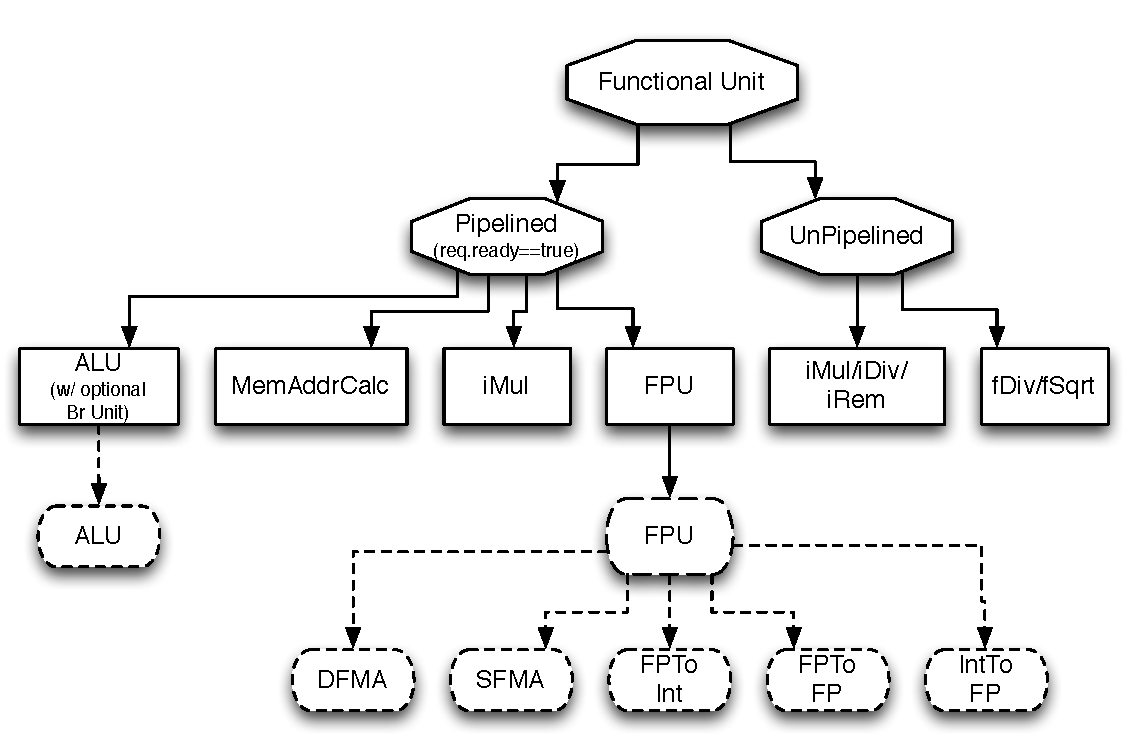
\includegraphics[scale =0.75] {figures/functional-unit-hierarchy}}
	\caption{ \small The dashed ovals are the low-level functional units written by experts, the squares are concrete classes that instantiate the low-level functional units, and the octagons are abstract classes that provide generic speculation support and interfacing with the BOOM pipeline.}
	\label{fig:functional-unit-hierarchy}
\end{figure}




\section{Branch Unit \& Branch Speculation}

The Branch Unit handles the resolution of all branch and jump instructions.  

All micro-ops that are ``inflight" in the pipeline (have an allocated ROB entry) are given a {\em branch mask}, where each bit in the {\em branch mask} corresponds to an un-executed, inflight branch that the micro-op is speculated under. Each branch in {\em Decode} is allocated a {\em branch tag}, and all following micro-ops will have the corresponding bit in the {\em branch mask} set (until the branch is resolved by the Branch Unit). 

If the branches (or jumps) have been correctly speculated by the front-end, then the Branch Unit's only action is to broadcast the corresponding branch tag to {\em all} inflight micro-ops that the branch has been resolved correctly.  Each micro-op can then clear the corresponding bit in its {\em branch mask}, and that branch tag can then be allocated to a new branch in the {\em Decode} stage. 

If a branch (or jump) is misspeculated, the Branch Unit must redirect the PC to the correct target, kill the front-end and fetch buffer, and broadcast the misspeculated {\em branch tag} so that all dependent, inflight micro-ops may be killed.  The PC redirect signal goes out immediately, to decrease the misprediction penalty.  However, the {\em kill} signal is delayed a cycle for critical path reasons. 

The front-end must pass down the pipeline the appropriate branch speculation meta-data, so that the correct direction can be reconciled with the prediction.  Jump Register instructions are evaluated by comparing the correct target with the PC of the next instruction in the ROB (if not available, then a misprediction is assumed).  Jumps are evaluated and handled in the front-end (as their direction and target are both known once the instruction can be decoded). 

% TODO{do jumps need to be in the pipeline at all? what about in-correct branch target exceptions?}

BOOM (currently) only supports having one Branch Unit. %Relaxing this constraint would add more ports to the ROB PC File. 

\section{Load/Store Unit}.

The Load/Store Unit (LSU) handles the execution of load, store, atomic, and fence operations. 

BOOM (currently) only supports having one LSU (and thus can only send one load or store per cycle to memory).\footnote{Relaxing this constraint could be achieved by allowing multiple LSUs to talk to their own bank(s) of the data-cache, but the added complexity comes in allocating entries in the LSU before knowing the address, and thus which bank, a particular memory operation pertains to.}

See Chapter \ref{sec:lsu} for more details on the LSU.

\section{Floating Point Units}

\begin{figure}[htbp]
	\centering
	\centerline{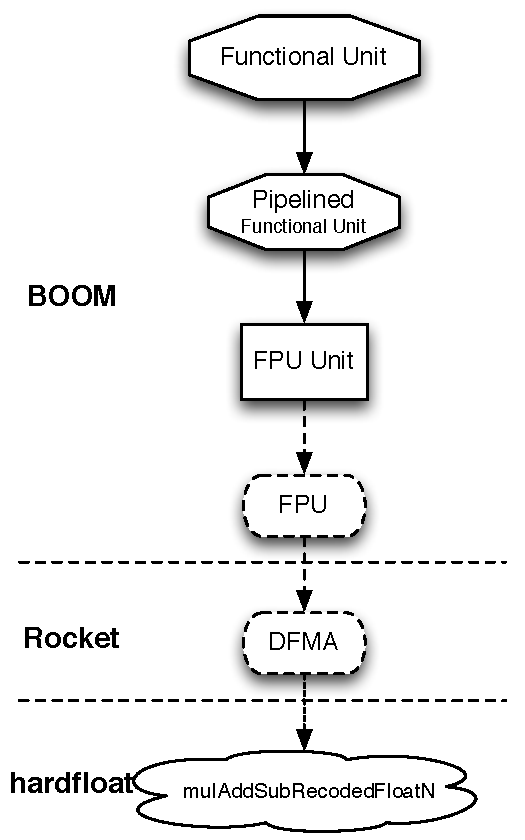
\includegraphics[scale =0.9] {figures/functional-unit-fpu}}
	\caption{ \small The class hierarchy of the FPU is shown. The expert-written code is contained within the {\tt hardfloat} and {\tt rocket} repositories. The ``FPU" class instantiates the Rocket components, which itself is further wrapped by the abstract Functional Unit classes (which provides the out-of-order speculation support).}
	\label{fig:functional-unit-fpu}
\end{figure}

The low-level floating point units used by BOOM come from the Rocket processor (\url{https://github.com/ucb-bar/rocket}) and hardfloat (\url{https://github.com/ucb-bar/berkeley-hardfloat}) repositories.  Figure \ref{fig:functional-unit-fpu} shows the class hierarchy of the FPU. 

To make the scheduling of the write-port trivial, all of the FP units are padded to have the same latency.\footnote{Rocket instead handles write-port scheduling by killing and refetching the offending instruction (and all instructions behind it) if there is a write-port hazard detected. This would be far more heavy-handed to do in BOOM.}



\section{Parameterization}

BOOM provides flexibility in specifying the issue width and the mix of functional units in the execution pipeline. Code \ref{code:exe_units} shows how to instantiate an execution pipeline in BOOM.
  
\begin{center}
\begin{minipage}{0.66\textwidth}
\begin{lstlisting}[caption=Instantiating the Execution Pipeline (in {\tt dpath.scala}). Adding execution units is as simple as instantiating another ExecutionUnit module and adding it to the {\tt exe\_units} ArrayBuffer.]
val exe_units = ArrayBuffer[ExecutionUnit]()

if (ISSUE_WIDTH == 2)
{
   exe_units += Module(new ALUExeUnit(is_branch_unit = true
                                       , has_mul     = true
                                       ))
   exe_units += Module(new ALUMemExeUnit(has_div     = true
                                       ))
}
else if (ISSUE_WIDTH == 3)
{
   exe_units += Module(new ALUExeUnit(is_branch_unit = true
                                       , has_mul     = true
                                       ))
   exe_units += Module(new ALUExeUnit(has_div = true))
   exe_units += Module(new MemExeUnit())
}
\end{lstlisting}\label{code:exe_units}
\end{minipage}
\end{center}

Additional parameterization, regarding things like the latency of the FP units can be found within the Configuration settings ({\tt configs.scala}).



\section{Control/Status Register Instructions}

A set of Control/Status Register (CSR) instructions allow the atomic read and write of the Control/Status Registers.  These architectural registers are separate from the integer and floating registers, and include the cycle count, retired instruction count, status, exception PC, and exception vector registers (and many more!).  Each CSR has its own required privilege levels to read and write to it and some have their own side-effects upon reading (or writing).  

BOOM (currently) does not rename {\em any} of the CSRs, and in addition to the potential side-effects caused by reading or writing a CSR, {\bf BOOM will only execute a CSR instruction non-speculatively.}\footnote{There is a lot of room to play regarding the CSRs. For example, it is probably a good idea to rename the {\tt sscratch} register (dedicated for use by the supervisor) as it may see a lot of use in some kernel code and it causes no side-effects.}  This is accomplished by marking the CSR instruction as a ``unique" (or ``serializing") instruction - the ROB must be empty before it may proceed to the Issue Window (and no instruction may follow it until it has finished execution and been committed by the ROB).  It is then issued by the Issue Window, reads the appropriate operands from the Physical Register File, and is then sent to the CSRFile.\footnote{The CSRFile is a Rocket component.}  The CSR instruction executes in the CSRFile and then writes back data as required to the Physical Register File. The CSRFile may also emit a PC redirect and/or an exception as part of executing a CSR instruction (e.g., a {\tt syscall}). 
